\section{\texorpdfstring{Kế hoạch triển khai}{Plan}}

Kế hoạch của Luận văn được chia thành các Task và được thực hiện theo giản đồ GANTT sau:

\begin{figure}[H]
    \centering
    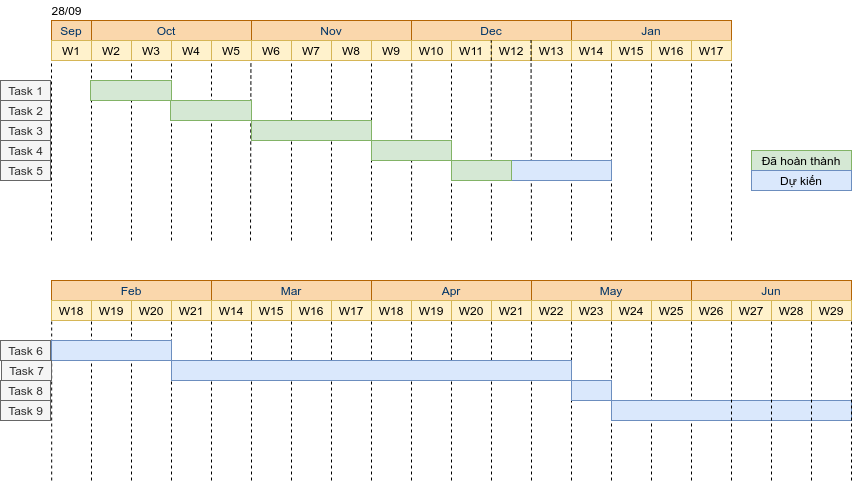
\includegraphics[width=15cm]{./content/images/gantt_chart.png}
    \caption{Kế hoạch thực hiện Luận văn}
    \label{fig:gantt_schedule}
\end{figure}

\textit{Task 1}: Tìm hiểu các kiến thức liên quan đến Variational Autoencoder và mạng GANs.

\textit{Task 2}: Tìm hiểu các kiến thức liên quan, ý tưởng, mô hình của nghiên cứu \cite{chen2018}. Đồng thời cài đặt và chạy thử mô hình.

\textit{Task 3}: Tìm hiểu các kiến thức liên quan, ý tưởng, mô hình của nghiên cứu \cite{vougioukas2019} và \cite{vougioukas2020}. Đồng thời cài đặt và chạy thử mô hình.

\textit{Task 4}: Tìm hiểu các kiến thức liên quan, ý tưởng, mô hình của nghiên cứu \cite{chen2019}. Đồng thời cài đặt và chạy thử mô hình.

\textit{Task 5}: Nghiên cứu các phương pháp tạo sinh ảnh dựa trên đặc trưng ba chiều bao gồm nghiên cứu của Lele chen vào năm 2020 \cite{chen2020}. Viết báo cáo và bảo vệ Đề cương Luận văn.

\textit{Task 6}: Tìm kiếm và tham khảo thêm các nghiên cứu tạo sinh hình ảnh có quan tâm đến cảm xúc tiếng nói.

\textit{Task 7}: Thiết kế, hiện thực và kiểm chứng các kiến trúc mạng mới.

\textit{Task 8}: Tổng hợp các thử nghiệm và lựa chọn kiến trúc tốt nhất cho Luận văn.

\textit{Task 9}: Viết báo cáo và bảo vệ Luận văn.
